\chapter{Results}
This chapter provides additional insight into the experimental results presented in the article proposal. Specifically, I will focus on providing additional explanations and presenting alternative methods, etc.

\section{Obfuscation method details}

\begin{table}[]
    \centering

    \begin{tabular}{llllllll}
\toprule
              &               &           &       &        &       &    &    \\
Type & Filter & Parameter & start & stop & num & step & val \\
\midrule
Constant & Gaussian noise & $\mu$ & NA & NA & NA & NA & 0.0 \\
\cline{2-8}
\multirow{2}{*}{Increments} & Mean filter & Kernel size & 1.00  & 51.00  & NA & 2.0 & NA \\
\cline{2-8}
              & Median filter & Kernel size & 1.00  & 51.00  & NA & 2.0 & NA \\
\cline{1-8}
\multirow{17}{*}{Interpolation} & \multirow{2}{*}{Bilateral filter} & $\sigma_c$ & 5.00  & 100.00 & 30.0  & NA & NA \\
              &               & $\sigma_s$ & 1.00  & 20.00  & 30.0  & NA & NA \\
\cline{2-8}
              & Cauchy noise & $\sigma$ & 1.00  & 50.00  & 100.0 & NA & NA \\
              \cline{2-8}
              & \multirow{3}{*}{Comb} & $\sigma$ & 1.00  & 50.00  & 20.0  & NA & NA \\
              &               & $\sigma_c$ & 10.00 & 60.00  & 10.0  & NA & NA \\
              &               & $\sigma_s$ & 1.00  & 20.00  & 10.0  & NA & NA \\
\cline{2-8}
              & \multirow{3}{*}{Comb Reverse} & $\sigma$ & 1.00  & 50.00  & 20.0  & NA & NA \\
              &               & $\sigma_c$ & 10.00 & 60.00  & 10.0  & NA & NA \\
              &               & $\sigma_s$ & 1.00  & 20.00  & 10.0  & NA & NA \\
\cline{2-8}
              & Gaussian filter & $\sigma$ & 0.00  & 50.00  & 100.0 & NA & NA \\
              \cline{2-8}
              & Gaussian noise & $\sigma$ & 0.00  & 100.00 & 100.0 & NA & NA \\
              \cline{2-8}
              & Laplacian noise & $\sigma$ & 0.00  & 100.00 & 100.0 & NA & NA \\
              \cline{2-8}
              & Non-local means & $h$ & 0.00  & 100.00 & 100.0 & NA & NA \\
              \cline{2-8}
              & \multirow{2}{*}{Salt-and-pepper noise} & Density & 0.01  & 0.99   & 15.0  & NA & NA \\
              &               & Intensity & 0.00  & 255.00 & 30.0  & NA & NA \\
\cline{2-8}
              & Snow noise & Density & 0.01  & 0.99   & 100.0 & NA & NA \\
              & Uniform noise & Intensity & 0.00  & 250.00 & 100.0 & NA & NA \\
\bottomrule
\end{tabular}


    \caption{Optimisation parameter overview.}
    \label{tab:parameters}
\end{table}

\section{Results}
\begin{figure}
	\centering
	
	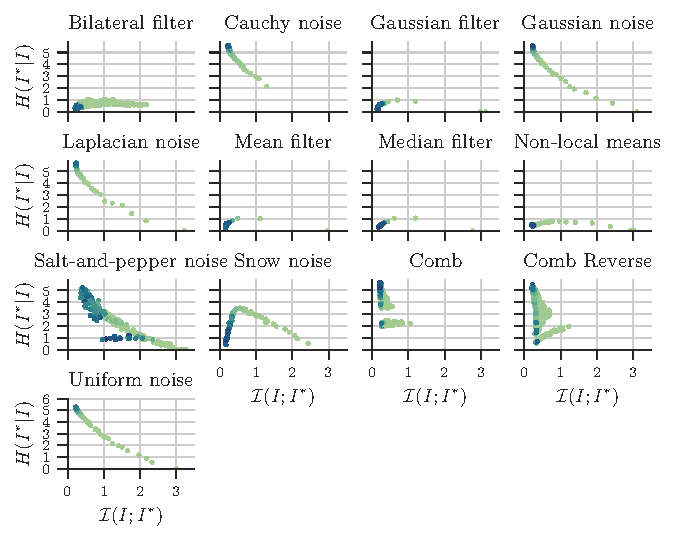
\includegraphics[width=1\textwidth]{figures/results/individual}
	
	\caption{Plot of mutual information and conditional information response for individual filters. Note that these distributions are estimated from the entire image, producing less noisy results than the ones presented in the article.}\label{fig:individual}
\end{figure}

\begin{figure}
	\centering
	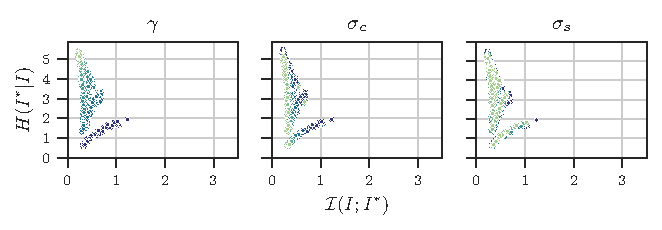
\includegraphics[width=1\textwidth]{figures/results/comb}
	\caption{}\label{fig:comb}
\end{figure}

\section{Additional performance considerations}